\documentclass{assignment}
\usepackage{amsmath}
\usepackage{lipsum}
\usepackage{multicol}
\usepackage{fancyhdr}
\usepackage{graphicx}
\usepackage{blindtext}
\usepackage[dvipsnames]{xcolor}
\usepackage{enumitem}
\usepackage{cleveref}
\usepackage{color,soul}
\usepackage{amsfonts}

\def\code#1{\texttt{#1}}
\newtheorem{anm}{Anm}

\begin{document}


\assignmentTitle
{Lucas Frykman}{0210127650}
{SF1930}
{Liam Solus}
{assets/KTH_logga.png}
{Statistisk inlärning och dataanalys}
{Projekt}

% \section*{Introduktion}
% Vi betraktar den skateboard tävlingen.

\section{Uppvärmning}
Figur för histogram för trick 1-4.

Låt $B$ vara betyg för en ett skateboardåkare och trick. Vi vill skatta $P(B>0.6|B>0) = \frac{P(B>0|B>0.6)P(B>0.6)}{P(B>0)}=\frac{P(B>0.6)}{P(B>0)}$
som $\tilde{P}(B>0.6|B>0) = \frac{\sum_{i}^4}{\sum_{j}^96}trick_{ij} = \indicator{A}$


\begin{figure}[!h]
    \caption{foo}
    \begin{center}
        % 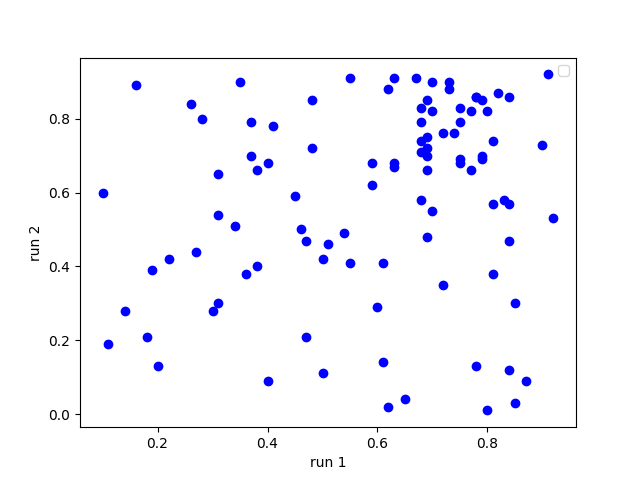
\includegraphics[width = 99mm]{assets/Figure_1.png}
        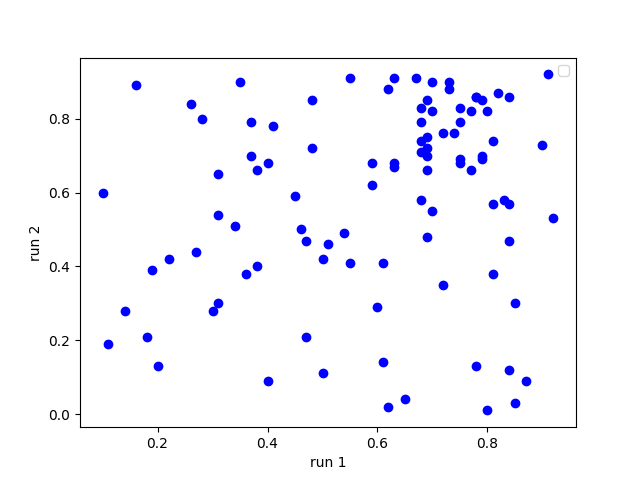
\includegraphics[width = 99mm]{assets/Figure_1.png}
    \end{center}
\end{figure}


\section{En frekventistisk modell}
\subsection*{(a) Skatta $\theta_{i}$}
Vi kan använda antingen momentmetoden eller ML metoden. Det går att visa att dessa två punktskattningar sammanfaller för $V_i \sim \text{Ber}(\theta_i)$.
Så vi använder momentmetoden för att skatta $\theta$ där
$m_1(\mathbf{X}) = \bar{X}$. Vi får punktskattningen för $\theta$ som
$m_1(\mathbf{x})= E[X|\tilde{\theta}] \Leftrightarrow \tilde{\theta} = m_1(\mathbf{x})$
\section{En bayesiansk modell}
\section{En bayesiansk modell med en hierarki}
\section{Diskussion}

% \section{Kod}
% \lstinputlisting[language=Matlab,caption=foo]{assets/tmp.m} 
\end{document}
